\documentclass[]{article}
\usepackage{amssymb}
\usepackage{amsmath}
\usepackage[utf8]{inputenc}
\usepackage{graphicx}
\usepackage{booktabs}
\usepackage{listings}
\usepackage{color}
\usepackage{tabularx}
\usepackage{hyperref}

\definecolor{dkgreen}{rgb}{0,0.6,0}
\definecolor{gray}{rgb}{0.5,0.5,0.5}
\definecolor{mauve}{rgb}{0.58,0,0.82}

\lstset{frame=tb,
	%language=C++,
	aboveskip=3mm,
	belowskip=3mm,
	showstringspaces=false,
	columns=flexible,
	basicstyle={\small\ttfamily},
	numbers=none,
	numberstyle=\tiny\color{gray},
	keywordstyle=\color{blue},
	commentstyle=\color{dkgreen},
	stringstyle=\color{mauve},
	breaklines=false,
	breakatwhitespace=true,
	tabsize=2
}


\title{FYS-STK4155 H20 - Project 3:\\Time Series Analysis with AR and RNN Models}
\author{Olav Fønstelien}

\begin{document}
\maketitle

\begin{abstract}
%The abstract gives the reader a quick overview of what has been done and the most important results. Try to be to the point and state your main findings. It could be structured as follows 
% - Short introduction to topic and why its important 
% - Introduce a challenge or unresolved issue with the topic (that you will try to solve) 
% - What have you done to solve this 
% - Main Results 
% - The implications

\end{abstract}

\section{Introduction} \label{sec:intro}
%When you write the introduction you could focus on the following aspects
% - Motivate the reader, the first part of the introduction gives always a motivation and tries to give the overarching ideas
% - What I have done
% - The structure of the report, how it is organized etc

% intro to condition monitoring of electric machines
% intro to insulation and temperature
% intro to transformers

Electric machines are highly reliable when properly designed and maintained. They are the workhorses in any industrial process, as well as the actuator in safety-critical functions, and failure may have both economic and physical consequences in the form of production downtime and personnel injury. Ensuring proper function of the machinery is a major cost driver in industry -- dedicated technicians are employed to execute detailed maintenance schedules while others log and monitor performance indicators like temperatures and vibration levels. Improving and automating such procedures is a large part of what \textit{Industry 4.0} is about. \textit{Digital twins} of the machines can be used to predict faults which are developing too slowly to be noticed, or which may not even be detectable with regular instrumentation. 

Machine learning methods play a central part in the development of digital twins. In this report we will see how a simple model for condition monitoring of the cooling system of an electric power transformer can be created by the use of traditional autoregression and more modern neural networks. Even small increases in a transformer's operating temperature may have severe effects on the lifetime of its electrical insulation, and ensuring that the cooling system performs as designed is vital for reliability and performance of the transformer. We will create model of the transformer which lets us evaluate the cooling system's performance under dynamic operating conditions based only on a few input measurements which are normally monitored in a standard plant automation and control system. The performance at the time of model creation will serve as the baseline against which future performance will be measured.

For developing this model we have available a dataset containing operational data of a power transformer -- an introduction of which is given further down in Section \ref{sec:case-description}. STRUCTURE OF REPORT [....], but first a short review of some power transformer essentials.


\subsection{Electric Power Transformer Basics} \label{sec:transformers}
Electrical power distribution networks usually have several voltage levels, and it is the power transformer's job to \textit{transform} the power from one voltage level to another. In a three-phase power system, each phase will be connected to separate transformer \textit{windings} -- one per phase for the high voltage (HV) side and one per phase for the low voltage (LV) side. The HV and LV windings of each phase are constructed like concentric cylinders with the ferromagnetic core in the middle for magnetic coupling between them. The phase windings again are physically separated from each other, but they are usually installed together either inside a tank containing cooling oil; or an air-filled enclosure, like the one we will treat in this report. 

A typical example of an air-cooled transformer is shown in Figure \ref{fig:dry-transformer}. The three phase windings, denoted $U, V, W$, are the red barrel-like structures seen inside the (opened) enclosure. The windings, usually made of copper or aluminium, develop heat when they conduct current. The phase windings are therefore constructed with a gap between the concentric HV and LV winding to allow air to flow between them for cooling. During operation the transformer is fully enclosed and air is circulated by the cooling fan motors, which we see on the outer wall to the upper left (blue-gray). The air is forced through the windings by the horizontal separation plate located close to the bottom of the windings. The heat dissipated by the windings is drawn out of the system by an air-water heat exchanger, which is located below the motors close to the floor. 

The winding insulation on this type of transformers is usually made of epoxy, which is mechanically robust and has good electric insulating properties. Epoxy consists of long hydrocarbon chains which has an exponential temperature-dependent degradation rate; a temperature increase of 6 kelvin approximately halves the useful lifetime of the material (\textit{Arrhenius' law}), so operational temperature is a major design parameter. Expected lifetime under nominal operating conditions is 180.000 hours ($\sim 20$ years) -- a number which however varies greatly between manufacturers and even otherwise identical units from the same manufacturer \cite{iec60076-12}.

The operation of the transformer is monitored by reading phase currents and winding temperatures, as well as the operational status of auxiliary systems like cooling fans. The measurements are transmitted to the plant automation and control system which monitors the condition of the transformer together with other equipment in the plant, and which may also store measurements digitally on a server. Refer to \cite{hubert2002} for an easy-to-read introduction to electric machines.

\begin{figure}[!h]
	\centering
	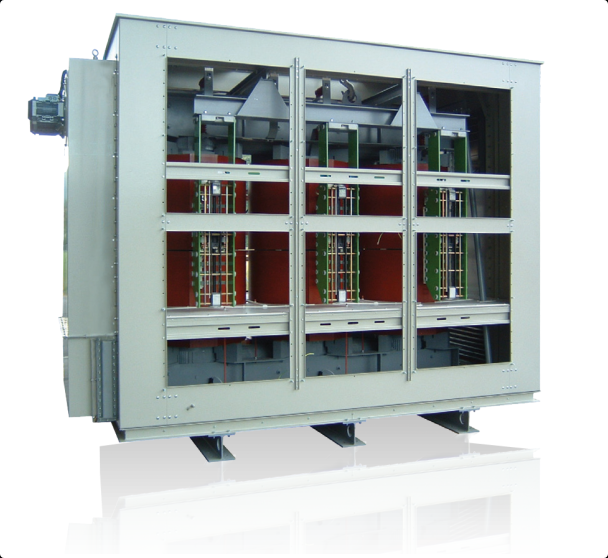
\includegraphics[width=1\linewidth]{./figs/dry-transformer.png}
	\caption{Typical air-cooled transformer with three phases $U, V, W$. The windings are the red barrel-like structures seen inside the cabinet, and the HV winding is placed within the LV winding as two concentric cylinders wrapped around the ferromagnetic core. Note that the transformer seen here is for illustrative purposes only and does not relate to the results in this report in any way.}
	\label{fig:dry-transformer}
\end{figure}

\subsection{Case Description} \label{sec:case-description}
For the design, training and testing of our transformer temperature model, we have a dataset provided by ABB AS \cite{abb-url}. The dataset contains operational data from a 12 MVA (mega volt-amperes) transformer as a time series stretching over approximately 14 months. Sampling rates are between 1 second and 1 minute, depending on the signal. The transformer serves an industrial process with a highly fluctuating demand; typically 2 hours of service at 40-80 \% load, with 30 minutes breaks in-between at 0 \%, as well as a 6 hours break at night-time. The cooling fans are usually turned off between the service intervals, but with a delay. See Figure \ref{fig:temp-current-aux}.

\begin{figure}[!h]
	\centering
	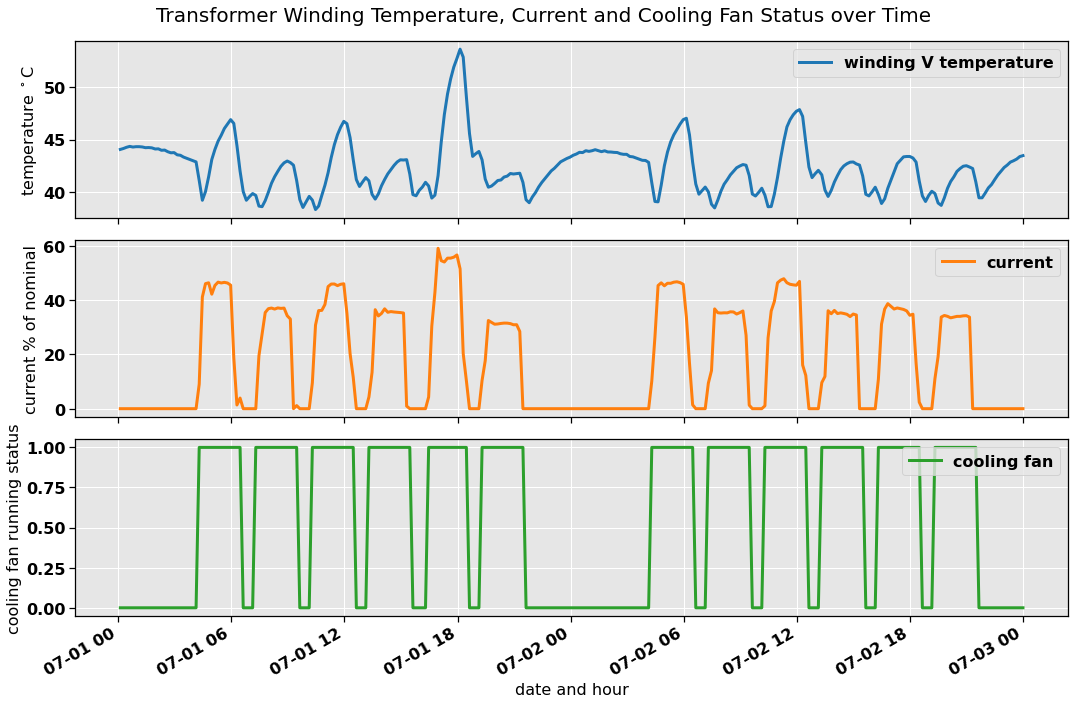
\includegraphics[width=1\linewidth]{./figs/temp-current-aux.png}
	\caption{Typical operational profile of the transformer with winding temperature (top), current (middle) and running status of the cooling fans (bottom, 1 = ON, 0 = OFF). The temperature-dependency on current is seemingly self-evident, but the cooling fan also plays a role as we see from the increase in temperature as both current and cooling fans are turned off.}
	\label{fig:temp-current-aux}
\end{figure}

The temperature in the three phase windings should not deviate much from each other in a well-designed transformer, but there will always be small differences, as we see in Figure \ref{fig:all-winding-temperature-over-time}. The 2-4 kelvin difference is caused by some variation in the air flow through the windings due to physical location within the enclosure and different shape of the ferromagnetic core at the center of the windings. Typically, the center winding will have slightly higher temperature than the others, corresponding to the $V$ winding in Figure \ref{fig:all-winding-temperature-over-time}. Another interesting observation is that the winding temperature curve turns upwards in the time after the cooling fans are shut off. Heat is coming into the windings, probably from the HV windings (we are looking at LV temperatures). Due to the higher demands to electrical insulation and therefore more complex construction, the HV windings are not monitored.

\begin{figure}[!h]
	\centering
	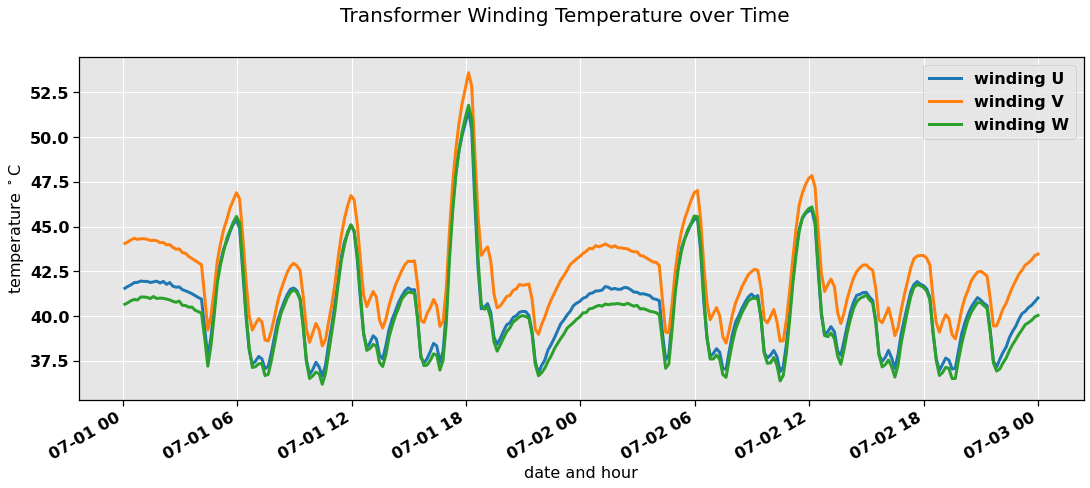
\includegraphics[width=1\linewidth]{./figs/all-winding-temperature-over-time.png}
	\caption{Development of the temperatures in windings $U,V,W$ of a healthy transformer. The temperatures follow each other closely only deviate a few degrees because of small difference in air flow through each winding.}
	\label{fig:all-winding-temperature-over-time}
\end{figure}


\section{Methods} \label{sec:methods}
% - Describe the methods and algorithms
% - You need to explain how you implemented the methods and also say something about the structure of your algorithm and present some parts of your code
% - You should plug in some calculations to demonstrate your code, such as selected runs used to validate and verify your results. The latter is extremely important!! A reader needs to understand that your code reproduces selected benchmarks and reproduces previous results, either numerical and/or well-known closed form expressions.

Failure or degradation of the transformer cooling system may take one of two forms -- either as an overall problem, which will present itself as increased operation temperature of the whole transformer; or as a failure affecting only one transformer phase winding, giving increased temperature in that winding. 

Common causes for the first would be reduced air flow due to a damaged impeller or oxidation inside the heat exchanger, which will reduce its efficiency. Especially oxidation is a slowly-developing fault which may be difficult to spot. To discover such developments, we need a fine-tuned model which precisely predicts the winding temperature in a healthy transformer in any operation condition. Deviation in actual temperature from the predicted temperature will then be indicative of a fault. For this \textit{Overall Temperature Model}, phase current and the running status of the cooling fans will be our input. The temperature of the water flowing into the heat exchanger as well as the room temperature would of course be highly valuable as well, but those measurements are not available in the data which we have.

The other type of fault, affecting only one of the three transformer windings, would typically be caused by mechanical obstruction of the air flow through the winding, for instance by an air guide which has come loose. For this \textit{Relative Temperature Model}, the temperature of the other windings will be the most important input, since they will be mostly unaffected by this. Again, deviation from the predicted temperature will be indicative of failure.

In the following, we will explore three different approaches for creating these models; first a physical model approach where we use what we know about heat dissipation in electrical conductors along with \textit{Newton's law of cooling}; then a traditional autoregressive (AR) model approach, which will yield equations which can easily be solved by the Ordinary Least Squares (OLS) method; and lastly by using recursive neural networks (RNNs), suitable for time series data.

\subsection{First Approach: Physical Models} \label{sec:physical-model}
We will treat the two parts of our temperature model separately. First we will look at the Overall Temperature Model, which shall predict the transformer temperature based on operational parameters; then we will look at the Relative Temperature Model, which shall predict the temperature of one winding based on the temperature of the two others.

\subsubsection{Physical Model: Overall Temperature} \label{sec:physical-model-overall}
The efficiency of air-cooled transformers usually lay in the 98-99 \% range. For the 12 MVA transformer studied here, that translates to some 120-240 MW. Most of the losses are due to electrical resistance in the windings and are dissipated as heat, which must be transported out through the cooling system. The resistance is temperature dependent, and within normal operating temperatures the heat dissipation at temperature $T$ is given by
\begin{equation}
\dot{Q}_T = I^2 [R + \alpha(T - T_0)],
\end{equation}
where $I$ is the current, $R$ is the resistance at reference temperature $T_0$ (usually 20 $^\circ$C) and $\alpha$ is the temperature coefficient for the material, which is $\sim 4 \cdot 10^{-3}$ $^\circ \text{C}^{-1}$ for copper and aluminium. 

Heat is removed from the transformer through the heat exchanger according to Newton's law of cooling;
\begin{equation}
	\dot{Q}_W = uK_W (T - T_W),
\end{equation}
where $T_W$ is the water temperature, and $K_W$ is some constant representing the efficiency of heat transfer from the winding, through the air and out of the heat exchanger. The factor $u$ represents the binary \textit{ON/OFF} running status of the cooling fans -- that is; $u \in \{0,1\}$. Heat is also removed through the walls of the transformer into the room. This relation can be stated as
\begin{equation}
	\dot{Q}_A = K_A (T - T_A),
\end{equation}
where $K_A$ is similar to $K_W$, and $T_A$ is the ambient temperature. Heat transfer from the windings to the heat exchanger and the room happens at a delay, since heat is also stored in the system. If we denote the total heat capacity of the transformer by $C$, the stored heat at temperature $T$ is given by $Q_S = CT$, such that the heat flow from the windings and out of the transformer is given by the power balance
\begin{equation} \label{eq:heat-flow-compact}
	\dot{Q}_T = C \dot{T} + \dot{Q}_W + \dot{Q}_A.
\end{equation}
Since we are dealing with time series here, it is natural to approximate $\dot{T}$ by its Taylor expansion $\dot{T}_{(t)} = (T_{(t)} - T_{(t-\Delta t)})/ \Delta t$. At time $t$, Equation (\ref{eq:heat-flow-compact}) solved for temperature $T_{(t)}$ then becomes
\begin{equation} \label{eq:physical-overall}
	T_{(t)} = \frac{\frac{C}{\Delta t} T_{(t-\Delta t)} + uK_W T_W + K_A T_A + I^2 (R - \alpha T_0)}{\frac{C}{\Delta t} + uK_W + K_A - I^2 \alpha}.
\end{equation}

At this point it is tempting to let the resistance temperature coefficient $\alpha = 0$, but normal operating temperature range for a transformer is 30-130 $^\circ$C, meaning that the resistive loss in the windings will vary by $\sim 100 \cdot 4 \cdot 10^{-3} = 40 $ \%, and any accurate model would have to account for this. Further, since we do not know $T_W$ and $T_A$, neither at $t = 0$ nor later, we could maybe assume that they could be held constant. This assumption, however, is likely to not be correct, since the heat from the transformer probably will increase the room temperature as well as the incoming water temperature, which runs in a closed circuit. In addition, in order to solve this model with traditional methods like the Ordinary Least Squares method to find $C, K_W, K_A$, we would have to linearize it -- which is not entirely straight-forward. We will therefore abandon this model, but the insights gained here will be useful when we design the features for our autoregressive and our neural network models.

\subsubsection{Physical Model: Relative Temperature} \label{sec:physical-model-relative}
In a healthy transformer, the temperature in any of the three windings will be closely linked to the temperature of the two others. Since the the electric impedance must be equal between the windings in order to maintain a balanced system voltage, we can assume that the electric losses will also largely be equally distributed in a well-designed transformer. Any difference in temperature is therefore likely to stem from small differences in the air flow through each winding. These assumptions correspond well with what we see in the winding temperature plots in Figure \ref{fig:all-winding-temperature-over-time}.

We will assume a linear relationship between the temperatures;
\begin{equation} \label{eq:physical-relative}
	T_X = K_{XY} T_Y + K_{XZ} T_Z,
\end{equation}
where $X,Y,Z$ may represent any one of the phase windings $U,V,W$. Given a time series with all three signals, this model can be solved easily with OLS.

\subsection{Second Approach: Autoregressive Models} \label{sec:autoregressive-model}
As for the physical in the previous section, we will make an Overall Temperature Model for the predicted temperature of the transformer based on the operation, and then a Relative Temperature Model for deviation between the windings. But first, let's take a moment to review the foundations of autoregression.

\subsubsection{A Brief Review of Autoregression} \label{sec:ar-review}
Autoregression (AR) is a statistical method made specifically for time series. It is based on the assumption that the $k$th value $y_{(k)}$ of a time series $y = \{y_{(0)}, y_{(1)}, ..., y_{(k)}, ...\}$ can be explained by a linear, weighted sum of its $p$ preceding values. Hence its name auto (self) regression. The process can be described as
\begin{equation} \label{eq:ar-basis}
	y_{(k)} = w_1 y_{(k-1)} + w_1 y_{(k-2)} + \cdots + w_p y_{(k-p)} + \varepsilon_{(k)} = \mathbf{w} \mathbf{y}_p + \varepsilon_{(k)}
\end{equation}
where the $\mathbf{w} = \{w_{i}\}$ are the weights, $\mathbf{y}_p = \{y_{(k-i)}\}_p$ are $y_{(k)}$'s $p$ preceding values, and $\varepsilon_{(k)} \sim \mathcal{N}(0,\sigma^2)$ is the process' noise. A model with $p$ terms such as Equation (\ref{eq:ar-basis}) would be referred to as a $p$th order AR model, or simply AR($p$). We can also introduce a vector of \textit{exogenous} variables $\mathbf{x}$ into this model -- that is; variables which are not decided within the system described by $y$. This model is sometimes called the ARX model and takes the form
\begin{equation} \label{eq:arx-basis}
	y_{(k)} = \mathbf{w}_y \mathbf{y}_p + \mathbf{w}_x \mathbf{x} + \varepsilon_{(k)}.
\end{equation}
Here, $\mathbf{x} = \{x_{i(k)}\}$, where $x_{i(k)}$ represents the $k$th value of the $i$th exogenous variable, and $\mathbf{w}_x = \{w_i\}_x$ are their weights. The "X" in ARX is often dropped, so the systems described in Equations (\ref{eq:ar-basis}) and (\ref{eq:arx-basis}) are both referred to as AR models. 

For the AR model to work, the time series must meet two requirements; it must be \textit{stationary} and \textit{ergodic}. Stationarity is met if the time series does not have an underlying trend, meaning that the expectation value of any two series of samples $y_1 = \{y_{(a)}, y_{(a+1)}, ..., y_{(b)}\}$, $y_2 = \{y_{(c)}, y_{(c+1)}, ..., y_{(d)}\}$ must be constant;
\begin{equation}
	\mathbb{E}(y_1) = \mathbb{E}(y_2) \Rightarrow \frac{1}{b-a} \sum_{i=a}^{b} y_{(i)} = \frac{1}{c-d} \sum_{i=c}^{d} y_{(i)}.
\end{equation}
The other criteria, that of ergodicity, is met if the \textit{autocovariance} falls to zero;
\begin{equation}
	\lim\limits_{j \rightarrow \infty} \mathrm{cov}(y_{(t)}, y_{(t-j)}) = 0.
\end{equation}
Relating this to Equations (\ref{eq:ar-basis}) and (\ref{eq:arx-basis}), this means that $w_q \approx 0$ for $q > p$. Refer to \cite{shumway2017} for a thorough treatment of statistical time series analysis.

The AR model weights $\mathbf{w}_y, \mathbf{w}_x$ are then found by linear regression methods, usually OLS. To do this, we must first arrange the time series $y$ and $x_i$ in a design matrix $\mathbf{X}$ and a target vector $\mathbf{y}$ such that they can be plugged into the OLS equation for optimal weight values;
\begin{equation} \label{eq:ols}
	\hat{\mathbf{w}} = (\mathbf{X}^\intercal \mathbf{X})^{-1} \mathbf{X}^\intercal \mathbf{y},
\end{equation}
where $\hat{\mathbf{w}} = [\hat{\mathbf{w}}_y \quad \hat{\mathbf{w}}_x]^\intercal$. If we denote the length of the time series by $n$, and the number of exogenous variables $m$, $\mathbf{X}$ will be on the form
\begin{equation}
\mathbf{X} = 
	\left[ 
	\begin{array}{ccccccc}
		y_{(p-1)} & y_{(p-2)} & \cdots & y_{(0)} & x_{1(p)} & \cdots &  x_{m(p)} \\
		y_{(p)}   & y_{(p-1)} & \cdots & y_{(1)} & x_{1(p+1)} & \cdots &  x_{m(p+1)} \\	
		\vdots  & \vdots  &          & \vdots  & \vdots   &        &  \vdots   \\
		y_{(n-2)} & y_{(n-3)} & \cdots & y_{(n-p-1)} & x_{1(n-1)} & \cdots &  x_{m(n-1)} \\			
	\end{array}
\right].
\end{equation}
Thus, we will discard the first $p$ values from each time series $y, x_i$ such that  $\mathbf{y} = [y_{(p)} \quad y_{(p+1)} \quad \cdots \quad y_{(n-1)}]^\intercal$. When we solve Equation (\ref{eq:ols}), we should probably use singular value decomposition of $\mathbf{X}$ and calculate its pseudoinverse to avoid any problems with singular matrices. See \cite{lay2016linear}.

After having found the optimal weights $\hat{\mathbf{w}}$, we will want to evaluate the model for some input time series $x_i$ of lengths $l$ and a given starting condition $y_0$. We will assume steady state initially, such that the predicted sequence $\mathbf{y}_{pred}$ becomes
\begin{equation}
\begin{aligned}
	&\mathbf{y}_{pred} = 
	\left[ 
\begin{array}{c}
	y_{(1)}	\\
	y_{(2)}	\\
	y_{(3)}	\\
	\vdots  \\
	y_{(p+2)}	\\
	\vdots  \\
	y_{(l)}	\\
\end{array}
\right]
	 \\
	&= \left[ 
		\begin{array}{ccccccc}
			y_{(0)} & y_{(0)} & \cdots & y_{(0)} & x_{1(1)} & \cdots &  x_{m(1)} \\
			y_{(1)} & y_{(0)} & \cdots & y_{(0)} & x_{1(2)} & \cdots &  x_{m(2)} \\	
			y_{(2)} & y_{(1)} & \cdots & y_{(0)} & x_{1(3)} & \cdots &  x_{m(3)} \\
			\vdots  & \vdots  &        & \vdots  & \vdots   &        &  \vdots   \\
			y_{(p+1)} & y_{(p)} & \cdots & y_{(1)}  \\
			\vdots  & \vdots  &        & \vdots     \\
			y_{(l-1)} & y_{(l-2)} & \cdots & y_{(l-p-1)} & x_{1(l)} & \cdots &  x_{m(l)} \\			
		\end{array}
	\right]
	\left[ 
\begin{array}{c}
w^{(y)}_1 \\
w^{(y)}_2 \\
\vdots \\
w^{(y)}_p \\
w^{(x)}_1 \\
\vdots \\
w^{(x)}_m \\
\end{array}
\right]	
\end{aligned}
\end{equation}
The model will thus have a run-up period of $p$ time steps, and a convergence time which depends on the system dynamics of the starting instance as well as the weights $\mathbf{w}_y$. If $y_{(0)}$ is unknown to us, we may pick a value at random or set it to zero, but the convergence time will then be longer. We also note that since the terms $y_{(t)}$ appear on both sides of the equation, $\mathbf{y}_{pred}$ must be calculated sequentially. 

\subsubsection{AR Model: Overall Temperature} \label{sec:ar-model-overall}
The autoregressive model encompasses a time-difference equation for the signal we want to model, and is as such a good starting point for modelling the overall transformer temperature, as shown in Equation (\ref{eq:physical-overall}). Following the discussion in Section \ref{sec:physical-model-overall}, we should expect that the exogenous variables going into the AR model in Equation (\ref{eq:arx-basis}) would be at least the current $I$ and the status of the cooling fans $u$, such that the temperature $T$ at time $t$ could be modelled as
\begin{equation} \label{eq:ar-overall-0}
	T_{(t)} = \sum_{i=1}^{p} w_i T_{(t-i)} + w_u u_{(t)} + w_{I} I_{(t)}.
\end{equation}
It would then be up to the $p$ time-difference terms to make up for the variables in Equation (\ref{eq:arx-basis}) which are not contained within $u,I$ during model fitting time -- that is; the water and room temperatures $T_W$ and $T_A$, in addition to the non-linear power loss due to $\alpha$. The cooling fan status is binary (ON/OFF), and as we observed from the winding temperature curves in in Figure \ref{fig:temp-current-aux}, heat is flowing into the winding for some time after the transformer and the cooling fans are shut down. To account for this in Equation (\ref{eq:ar-overall-0}), we can add a term $u' = 1 - u$, such that
\begin{equation}
	w_u u_{(t)} + w_{u'} u'_{(t)} = (w_u - w_{u'})u + w_{u'},
\end{equation}
which really amounts to adding an intercept, which we will denote by $w_0$. Further, looking at the current we know that temperature is more likely to depend on the power loss in the windings, which is closer related to the current squared; $I^2$. Replacing $I$ with $I^2$ yields the equation for our AR($p$) model
\begin{equation} \label{eq:ar-overall-1}
	T_{(t)} = w_0 + \sum_{i=1}^{p} w_i T_{(t-i)} + w_u u_{(t)} + w_{I} I^2_{(t)}.
\end{equation}
The optimal weights and model order $p$ will then be determined by OLS in an iterative process.

\subsubsection{AR Model: Relative Temperature} \label{sec:ar-model-relative}
For the relative temperature model we already derived the exogenous variables in Section \ref{sec:physical-model-relative}. We will simply install the terms in Equation (\ref{eq:physical-relative}) in the general AR model in Equation (\ref{eq:arx-basis});
\begin{equation} \label{eq:ar-relative}
	T_{(t)} = \sum_{i=1}^{p} w_i T_{(t-i)} + w_X T_{X(t)} + w_Y T_{Y(t)}.
\end{equation}
Again, we expect the $p$ time-difference terms to make up for any variables not contained within the temperatures of the other windings, $T_X, T_Y$.

\subsection{Third Approach: Recurrent Neural Network Models} \label{sec:neural-model}
Recurrent Neural Networks (RNNs) are a special class of neural networks designed for taking advantage of the time-proximity of sequential data when they make predictions. Like the simpler nodes in Feed Forward Neural Networks (FFNNs), RNN nodes sums all their inputs and adds a bias before applying an activation function like \textit{tanh}, \textit{sigmoid}, or similar. What distinguishes RNN nodes, however, is that they have a feedback loop such that the output resulting from the former input is \textit{remembered} by the node;
\begin{equation} \label{eq:rnn-node}
	\tilde{y}_{(t)} = f(w_x x_{(t)} + w_y \tilde{y}_{(t-1)} + b),
\end{equation} 
where $\tilde{y}_{(t)}$ and $x_{(t)}$ are the RNN node output and input at time $t$, $\tilde{y}_{(t-1)}$ is the node's preceding output. As for FFNNs, the learning parameters $b$ (bias) and the $w_x, w_y$ (weights) are incrementally optimized by back-propagation, but through time using some cost function $\mathcal{C}(y, \tilde{y})$ which is evaluated on the predicted sequence $\tilde{y} = \{\tilde{y}_{(0)}, \tilde{y}_{(1)}, ...\}$ against a target sequence $y = \{y_{(0)}, y_{(1)}, ...\}$.

Like for FFNNs, more complex patterns can be learned by letting parallel nodes form a layer. In such a structure, the output of each layer forms a vector which is fed back into each node of the layer. This way, even more complex structures can be remembered from earlier inputs. We can also let the input be a vector, containing one or more features. Equation (\ref{eq:rnn-node}) re-written for the whole layer then becomes
\begin{equation} \label{eq:rnn-layer}
	\mathbf{y}_{(t)} = f(\mathbf{w}_x \mathbf{x}_{(t)} + \mathbf{w}_y \mathbf{y}_{(t-1)} + \mathbf{b}),
\end{equation} 
where we have dropped the tilde to indicate predicted values.

and stacking layers on top of each other to form a deep neural network. 

back-propagation through time

\subsubsection{RNN Model: Overall Temperature} \label{sec:rnn-model-overall}

\subsubsection{RNN Model: Relative Temperature} \label{sec:rnn-model-relative}

\subsection{Data Preparation} \label{sec:data-prep}



\subsection{Subsection} \label{sec:subsection-name}
% The first part deals with structuring and reading the data, much along the same lines as done in projects 1 and 2. Explain how the data are produced and place them in a proper context. 




% You need to include at least two central algorithms, or as an alternative explore methods from decisions tree to bagging, random forests and boosting. Explain the basics of the methods you have chosen to work with. This would be your theory part. 

% Then describe your algorithm and its implementation and tests you have performed. 







\section{Results} \label{sec:results}
% - Present your results
% - Give a critical discussion of your work and place it in the correct context.
% - Relate your work to other calculations/studies
% - An eventual reader should be able to reproduce your calculations if she/he wants to do so. All input variables should be properly explained.
% - Make sure that figures and tables should contain enough information in their captions, axis labels etc so that an eventual reader can gain a first impression of your work by studying figures and tables only.

% Then presents your results and findings, link with existing literature and more. 


AR model: show stationarity and ergodicity

\section{Discussion and Conclusion} \label{sec:conclusion}
% - State your main findings and interpretations
% - Try as far as possible to present perspectives for future work
% - Try to discuss the pros and cons of the methods and possible improvements

% Finally, here you should present a critical assessment of the methods you have studied and link your results with the existing literature. 

validation of model by lab tests

may still fail even if perfectly maintained and monitored - ref bathtub curve

why not run transformer until it gets warm and use that for benchmarking -- may not be practicable or even possible in a real industrial application

\clearpage
\vspace{5mm}

%\clearpage
\bibliographystyle{unsrt}
\bibliography{project3.bib}
\end{document}
